\chapter*{chapter 3}
\markboth{Chapter 3 }{ Hardware and software system design } %pour afficher l'entete
 \addcontentsline{toc}{chapter}{III   Hardware and software system design }

\textbf{\Huge Hardware and software system design} 

\setcounter{chapter}{3}
\setcounter{section}{0}


\section{Introduction}
This chapter describes the design and implementation of the proposed simultaneous multi-
frequency EIT system. The process of development includes signal specification, hardware
design, PCB development, and firmware implementation on the STM32G4 platform. The
design should possess a high temporal resolution and accurate impedance measurements
through optimized multisine excitation and high-resolution 16-bit ADC sampling.
\section{Excitation signal specification}
In the proposed system, the excitation waveform is a \textit{multisine} signal generated by superimposing sinusoidal components at carefully selected frequencies. The selection of frequency values, frequency spacing, and amplitudes directly influences measurement precision, spectral range, and ability to follow impedance variations over a large bandwidth.
To verify performance, two configurations were employed and tested:
\begin{itemize}
    \item \textbf{Two-frequency multisine:} Reduced spectral coverage, used primarily for first-stage validation of the acquisition chain.
\item \textbf{Five-frequency multisine:} Sufficient coverage with less complexity, offering a compromise
towards the speed of measurement and spectral resolution.
\end{itemize}
For every configuration, the frequencies were selected in order to minimize harmonic overlap and intermodulation distortion, subject to the IEC 60601 amplitude limit requirements for biomedical safety.


\noindent
The generation of the excitation signal follows the algorithm illustrated in Figure~\ref{fig:multisine_algorithm}, implemented using a dedicated Python script.

\begin{figure}[H]
    \centering
    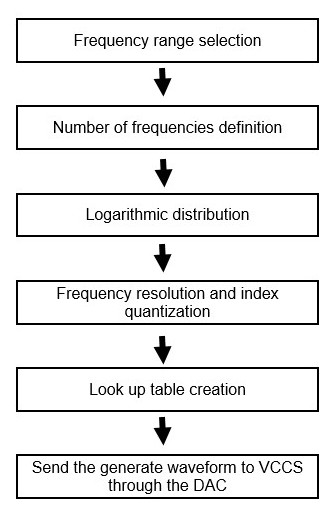
\includegraphics[width=0.4\linewidth]{imagess/Slide2.jpg}
    \caption{Flowchart of the multisine excitation signal generation process}
    \label{fig:multisine_algorithm}
\end{figure}

\subsection{Mathematical formulation of the excitation signal generation algorithm}
The procedure for generating the excitation signal consists of the following main steps:

\paragraph{Step 1: Frequency range definition}\\
The minimum and maximum frequencies are defined as: f_{\min}, \; f_{\max}


\paragraph{Step 2: Logarithmic frequency spacing}\\
For a total of \( N_{\text{freq}} \) frequencies, the logarithmic distribution is computed as:
\begin{equation}
f_k = f_{\min} \cdot \left( \frac{f_{\max}}{f_{\min}} \right)^{\frac{k}{N_{\text{freq}}-1}}, \quad k = 0, 1, \dots, N_{\text{freq}}-1
\label{eq:log_spacing}
\end{equation}

\paragraph{Step 3: Frequency quantization to FFT bins}\\
Considering a sampling frequency \( f_s \) and FFT length \( N_{\text{FFT}} \), the frequency resolution is:
\begin{equation}
\Delta f = \frac{f_s}{N_{\text{FFT}}}
\label{eq:delta_f}
\end{equation}
Each frequency is quantized to the nearest FFT bin:\\
\begin{equation}
f_k^{(q)} = \text{round}\left( \frac{f_k}{\Delta f} \right) \cdot \Delta f
\label{eq:quantization}
\end{equation}

\paragraph{Step 4: Multisine signal synthesis}\\
The discrete-time multisine signal is:
\begin{equation}
x[n] = \sum_{k=0}^{N_{\text{freq}}-1} A_k \cdot \sin\left( 2\pi \frac{f_k^{(q)}}{f_s} n + \phi_k \right)
\label{eq:multisine}
\end{equation}
where \( A_k \) is the amplitude of the \( k \)-th component and \( \phi_k \) is a random initial phase.

\paragraph{Step 5: Amplitude normalization and DAC mapping}\\
The signal is normalized to the DAC range \([0, 2^{N_{\text{bits}}} - 1]\):
\begin{equation}
x_{\text{DAC}}[n] = \left\lfloor \frac{x[n]}{\max |x[n]|} \cdot \left(2^{N_{\text{bits}}-1} - 1\right) + 2^{N_{\text{bits}}-1} \right\rfloor
\label{eq:dac_mapping}
\end{equation}
For the 12-bit DAC used in this work: \( N_{\text{bits}} = 12 \).


\paragraph{Step 6: LUT generation}\\
The final samples are stored in both CSV format and C header files for direct microcontroller integration.

\subsection{Component selection and justification}
The following table summarizes the key hardware components selected for the system, along with a brief description and justification for their inclusion.

\begin{table}[H]
\centering
\caption{Hardware component selection and justification}
\begin{tabular}{|p{4cm}|p{5cm}|p{7cm}|}
\hline
\textbf{Requirement} & \textbf{Selected component} & \textbf{Justification} \\
\hline
Low-noise precision amplification & ADA4610-2ARZ (Analog Devices) & Offers ultra-low input bias current (1 pA), low offset (50 $\mu$V), and low noise density (3 nV/$\sqrt{\text{Hz}}$), which is critical for microvolt-level EIT boundary voltage measurements\cite{ada4610}.\\
\hline
Scalable electrode switching & CD74HC4067SM96(Texas Instruments) & 16-channel analog multiplexer (16:1) with low ON resistance ($\sim$70 $\Omega$). Provides wide analog bandwidth ($\sim$89 MHz, $-3$ dB) suitable for the maximum excitation frequency of 2.5 MHz ($f_{\text{MUX}} \geq 2 \cdot N \cdot f_{\text{exc,max}}$), This ensures minimal distortion and correct per-channel sampling\cite{cd74hc4067}.\\

\hline
\end{tabular}
\end{table}
\begin{table}[H]
\centering
\begin{tabular}{|p{4cm}|p{5cm}|p{7cm}|}
\hline
\textbf{Requirement} & \textbf{Selected component} & \textbf{Justification} \\
\hline
Signal generation, acquisition, and control & STM32G474RE (STMicroelectronics) & Integrated high-speed ADC (up to 4 MSPS, 12-bit). Supports DMA for efficient data acquisition and multiple GPIOs for multiplexer control. Chosen due to its superior analog performance, processing capability, and robust development ecosystem (CubeMX, HAL, STM32 IDE)\cite{stm32g474re}. \\
\hline
Stable current excitation & Modified dual Howland VCCS with AD8021 op-amp & Provides stable AC currents (≤0.4 mA peak) across 50 kHz–1 MHz and 100 Ω–18 kΩ loads. Low-power design (5 V supply, 210 mW) ensures compliance with IEC-60601 safety standards. Supports multisine excitation, maintaining stability, enhancing accuracy and portability for wearable EIT applications\cite{ouni2024}.\\
\hline
\end{tabular}
\end{table}


\section{EIT circuit simulation on LTspice}
\label{sec:eit-ltspice}

Before investing in hardware, the EIT acquisition chain was verified with LTspice using
a controlled "known-resistor" device-under-test (DUT) rather than biological tissue or
the salt tank. This process validates the path of excitation, the analog front-end, and the
impedance extraction algorithm (voltage and current measurement), with the aim that
computed resistance is equivalent to the DUT component across the operating bandwidth.The full LTspice schematic of the simulated acquisition circuit is shown in Figure 3.9.

\begin{figure}[H]
    \centering
    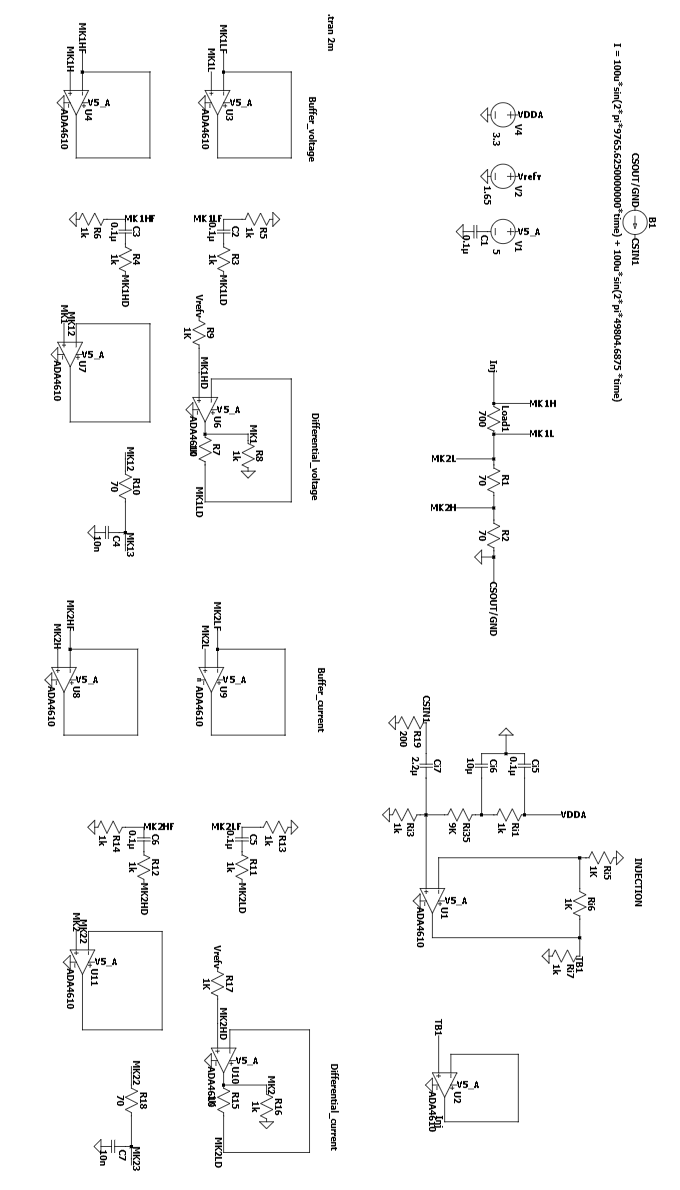
\includegraphics[width=0.8\textwidth]{imagess/LTspice_circuit.png}
    \caption{LTspice schematic of the simulated EIT acquisition circuit.}
    \label{fig:ltspice}
\end{figure}


\subsection{Excitation signal conditioning:}  
As shown in figure 3.10 the input excitation current $I_{\text{CSIN1}}$ is first converted into a small voltage by the resistor $R_{19}=200~\Omega$, yielding an AC voltage of approximately $100~\text{mV}$ peak for a $500~\mu\text{A}$ input. 
This AC signal is then coupled through $C_7=2.2~\mu\text{F}$, which blocks any DC component.\\
In this project, the EIT system is used to reconstruct the conductivity distribution of certain biomedical tissues, and its performance will be validated
with a water tank experiment. Since the conductivity profiles of the DUTs
are very different, a special excitation signal adjustment circuit is required.
The purpose of this circuit is to maintain the excitation signal within the
range so that the resulting output falls within the compatibility range of the amplifier input window and to scale both the DC
and AC components of the signal accordingly.
A resistive divider biases this AC signal to a suitable DC level. 
The resistors are defined as:  
\[
R_{i35} = 9~\text{k}\Omega, \quad R_{i1} = R_{i3} = 1~\text{k}\Omega
\]
With a supply voltage $V_{DDA} = 3.3~\text{V}$, the DC bias voltage at the junction of $R_{i1}$, $R_{i3}$ and $R_{i35}$ is:

\begin{equation}
    V_{DC} = V_{DDA} \cdot \frac{R_{i1}}{R_{i3} + R_{i35}}
\end{equation}

Substituting the values:  

\[
V_{DC} = 3.3 \cdot \frac{1~\text{k}\Omega}{1~\text{k}\Omega + 9~\text{k}\Omega} 
= 3.3 \cdot \frac{1}{10} 
= 0.33~\text{V}
\]  

This means the excitation signal is shifted to approximately $0.33~\text{V}$ DC. 
The AC amplitude is then adjusted by the amplification stage.

As shown in the figure, the op-amp (ADA4610) is configured as a non-inverting amplifier with the feedback resistors:  
\[
R_{i5} = R_{i6} = 1~\text{k}\Omega
\]

The gain is given by:  
\begin{equation}
G_1 = 1 + \frac{R_{i5}}{R_{i6}}
\end{equation}

Thus, the amplification factor is $G_1 = 2$, doubling the AC component while preserving the DC bias. 
Finally, the signal is passed to a unity-gain buffer stage, which provides the necessary drive capability for safe electrode injection without loading the adjustment circuit.
The buffer gain is ideally:
    G_{\mathrm{buf}} \approx 1.

\subsection{AC coupling and biasing (per channel)}
The boundary electrode voltages $V_{\text{in1}}$ and $V_{\text{in2}}$ are first buffered
by unity-gain amplifiers (ADA4610) to provide high input impedance and prevent
loading of the electrodes. The buffered signals are then AC-coupled through
capacitors $C_{2}$ and $C_{3}$.

Each capacitor, together with its associated resistor pair, forms a first-order
high-pass filter: $(C_{2},R_{5},R_{3})$ for the upper channel and
$(C_{3},R_{4},R_{6})$ for the lower channel. These filters block DC electrode
offsets and pass only the AC components of interest. The general transfer
function of each filter is

\begin{equation}
  H_{\mathrm{HP}}(j\omega) = \frac{j\omega R_{\mathrm{eq}} C}{1 + j\omega R_{\mathrm{eq}} C},
  \qquad f_c = \frac{1}{2\pi R_{\mathrm{eq}} C},
\end{equation}

where $R_{\mathrm{eq}}$ is the effective resistance seen by the capacitor. For
$R=1~\text{k}\Omega$ and $C=0.1~\mu\text{F}$, we obtain

\[
f_c = \frac{1}{2 \pi \cdot 1~\text{k}\Omega \cdot 0.1~\mu\text{F}}
     \approx 1.59~\text{kHz}.
\]

Because both channels use identical RC values, the two filters are matched in
gain and phase, which ensures accurate differential subtraction in the next
stage.



  
\subsection{Differential boundary voltage measurement}

The filtered signals are then applied to a differential amplifier with matched resistor ratios (feedback resistor $R_7$ and input resistor $R_9$), the transfer function can be written as

\begin{equation}
V_{\mathrm{out}} \;=\; \frac{R_7}{R_9}\,\bigl(V_{\text{in2}} + V_{\mathrm{ref}} - V_{\text{in1}}\bigr),
\end{equation}

where $V_{\text{in2}}$ and $V_{\text{in1}}$ are the two measurement nodes of the DUT and $V_{\mathrm{ref}}$ is a DC offset applied to shift the amplifier output into the ADC input range.

With $R_7 = R_9 = 1~\text{k}\Omega$ (matched resistors), the differential gain is unity:

\begin{equation}
G_{\mathrm{diff}} \;=\; \frac{R_7}{R_9} \;=\; 1,
\end{equation}

so the expression simplifies to
\begin{equation}
V_{\mathrm{out}} \;=\; V_{\text{in2}} - V_{\text{in1}} + V_{\mathrm{ref}}.
\end{equation}

Here, $V_{\mathrm{ref}} = 1.65\ \text{V}$ is chosen because it is the midpoint of the ADC input range (3.3~V). This centers the amplifier output around mid-scale, allowing small bipolar differential voltages $(V_{\text{in2}}-V_{\text{in1}})$ to be measured without saturating the ADC:

\begin{equation}
V_{\mathrm{out}} \;=\; V_{\text{in2}} - V_{\text{in1}} + 1.65\ \text{V}.
\end{equation}
Figure~\ref{fig:eit_injection1} illustrates the excitation adjustment stage along with the differential boundary voltage measurement circuit, which ensures that the injected signal remains within the ADC input range while accurately capturing the small voltage differences across the DUT
\begin{figure}[H]
    \centering
    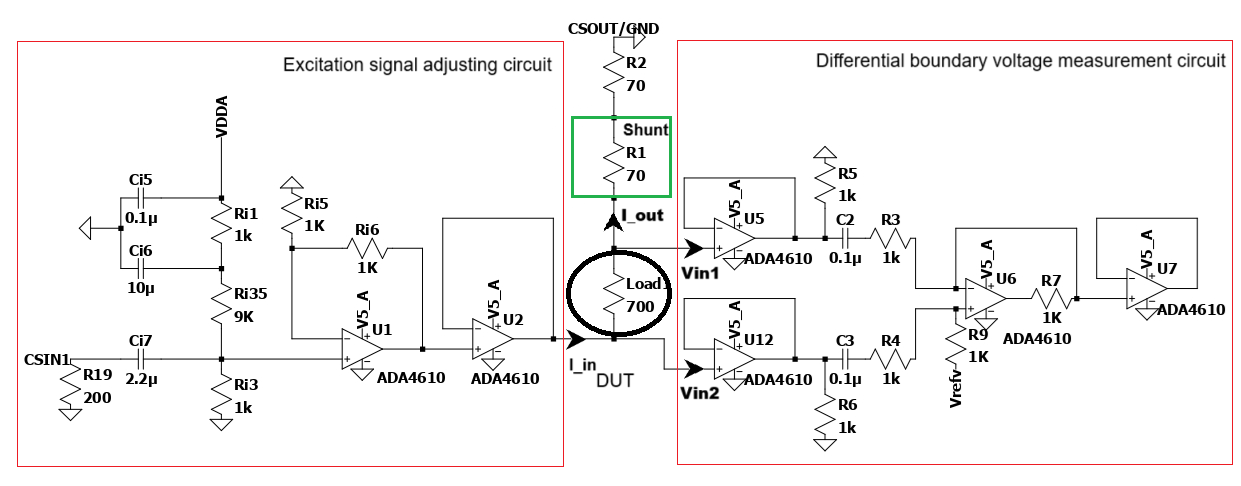
\includegraphics[width=1\linewidth]{imagess/injection_differentiaal.png}
    \caption{Excitation signal adjusting and differential boundary voltage measurement circuit}
    \label{fig:eit_injection1}
\end{figure}

\subsection{Differential current measurement circuit}  
In addition to boundary voltage acquisition, the injected current across the DUT must also be properly measured for impedance extraction. The same signal conditioning principle is applied:
first, the minor voltage drop on the precision shunt resistor ($R_{\text{shunt}}$) is buffered to provide high input impedance, and then similar high-pass filters are also used to guarantee that no DC component is delivered to the tissue. Then a differential amplifier stage suppresses common-mode
noise and extracts the actual shunt voltage.
For the traditional difference amplifier configuration with matched resistors (feedback
resistor $R_13$ and input resistor $R_17$), the transfer function is represented by



\begin{equation}
V_{\mathrm{out,\,I}} \;=\; \frac{R_{13}}{R_{17}}\,\bigl(V_{+} - V_{-} + V_{\mathrm{ref}}\bigr)
\end{equation}


where $V_{+}$ and $V_{-}$ are the voltages across the shunt resistor, and $V_{\mathrm{ref}}$ is the same DC offset (1.65~V) used to center the output within the ADC input range.

With $R_13 = R_17 = 1~\text{k}\Omega$, the differential gain is unity:

\begin{equation}
G_{\mathrm{diff}} \;=\; \frac{R_13}{R_17} \;=\; 1,
\end{equation}

and the expression simplifies to

\begin{equation}
V_{\mathrm{out,\,I}} \;=\; V_{+} - V_{-} + V_{\mathrm{ref}}.
\end{equation}

Since $V_{+}-V_{-}$ corresponds to the voltage drop across $R_{\text{shunt}}$, the output directly reflects the instantaneous current, shifted by the reference offset:

\begin{equation}
I_{\text{DUT}} \;=\; \frac{V_{+} - V_{-}}{R_{\text{shunt}}}, \qquad
V_{\mathrm{out,\,I}} \;=\; I_{\text{DUT}} \cdot R_{\text{shunt}} + V_{\mathrm{ref}}.
\end{equation}

This configuration ensures that both voltage and current measurement channels share the same architecture (buffering stage followed by differential amplification), providing high common-mode rejection, symmetry in signal processing, and robust performance in noisy environments.
  
Figure~\ref{fig:current_measurement_circuit} shows the practical realization of the current measurement circuit. The buffered differential amplifier processes the shunt voltage and outputs a mid-scale referenced signal suitable for digitization by the ADC. The layout mirrors the voltage measurement circuit, thereby simplifying design complexity and improving overall noise immunity.

\begin{figure}[H]
    \centering
    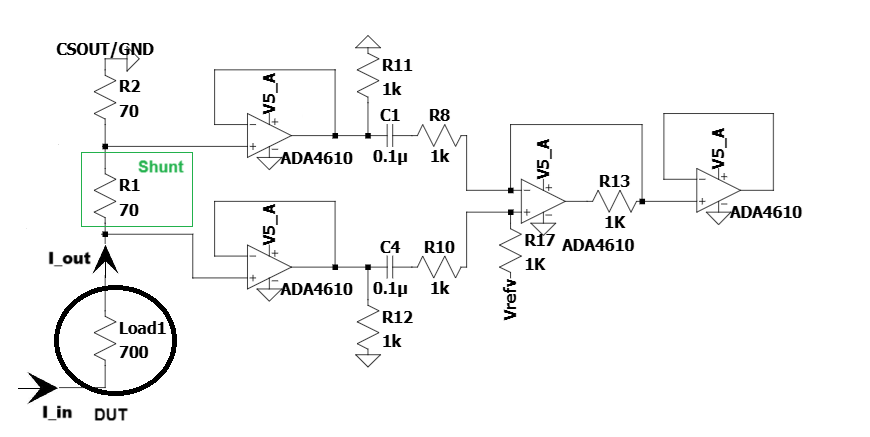
\includegraphics[width=1\textwidth]{imagess/Untitled (Recovered).png}
    \caption{Schematic of the current measurement circuit based on buffering and differential amplification.}
    \label{fig:current_measurement_circuit}
\end{figure}

   
\end{enumerate}

\subsection{Excitation and simulation settings}

\begin{itemise}
    \item \textbf{Load modeling:}  
Instead of the actual water tank with a metallic inclusion, the Device Under Test (DUT) 
was represented by a known resistor $R_{\text{load}}$. This substitution enables the 
verification of whether the simulation can recover the expected resistance value from 
the measured voltage and current. For example, when $R_{\text{load}} = 1~k\Omega$, the 
simulation should return a measured resistance close to $1~k\Omega$.

\item \textbf{Shunt resistor:}  
A shunt resistor $R_{\text{shunt}}$ of $70~\Omega$ was placed in series with the DUT 
to allow current measurement. The voltage drop across the shunt is processed by the 
current-differential amplifier in the real system. The choice of $70~\Omega$ represents 
a compromise: it is large enough to generate a measurable voltage drop for the amplifier 
while remaining small enough to avoid significantly perturbing the injected current.  
The instantaneous current through the DUT is thus obtained as : 

\begin{equation}
I_{\text{measured}}(t) = \frac{V_{\text{shunt}}(t)}{R_{\text{shunt}}}.
\end{equation}
\end{itemise}
The simulation was run in transient mode over a duration of $2~ms$, sufficient to capture 
multiple cycles of both excitation frequencies. 

Finally, the resistance was computed using the ratio of the measured voltage to the 
calculated current:
\begin{equation}
R_{\text{calculated}} = \frac{V_{\text{DUT}}}{I_{\text{measured}}}.
\end{equation}

\subsection{Results visualization and resistance calculation.}  



\paragraph{(A) Time-Domain Verification Using Single-Frequency Excitation}
The figure~\ref{fig:eit_injection} illustrates the injected current after passing through the injection circuit. A current source with the expression :
\begin{equation}
I(t) = 100~\mu A \cdot \sin(2\pi \cdot 9765.625 \cdot t) 
\end{equation}
(single-frequency) was used, and the plot shows the resulting waveform of the injected current.
\begin{figure}[H]
    \centering
    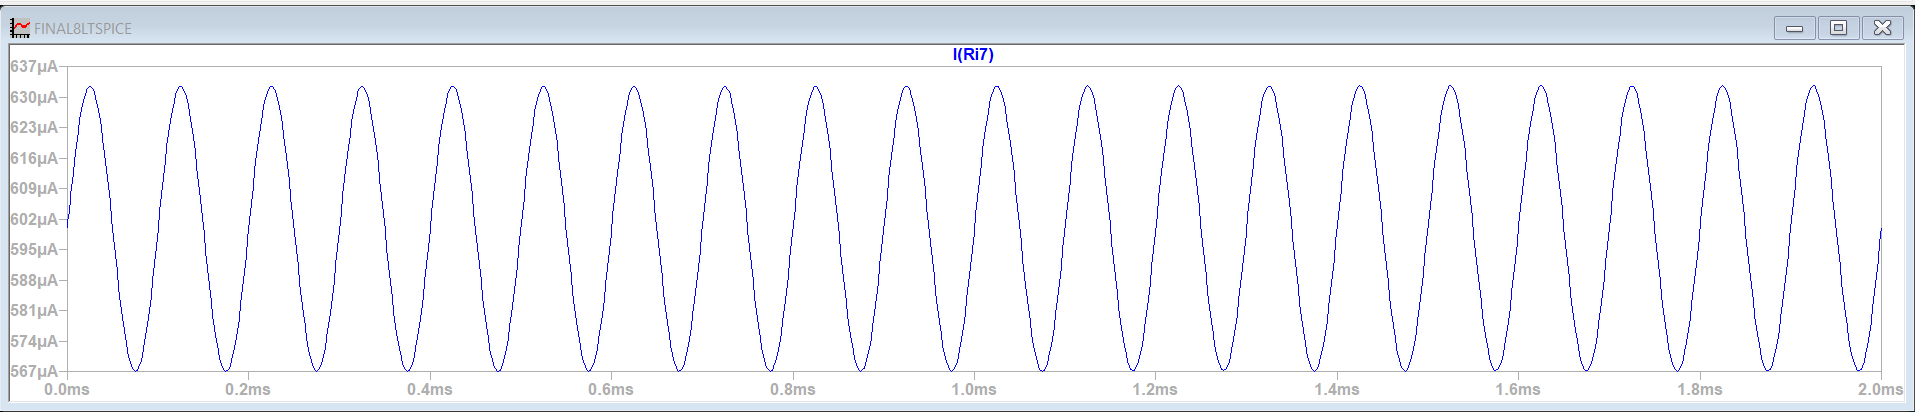
\includegraphics[width=1\linewidth]{imagess/Inj.png}
    \caption{Measured DUT current waveform obtained via shunt calculation.}
    \label{fig:eit_injection}
\end{figure}


\noindent Figures~\ref{fig:eit_voltage} and~\ref{fig:eit_current} present the measured 
voltage and current waveforms respectively. These plots confirm that both signals follow 
the expected sinusoidal behavior dictated by the sinewave excitation source.

\begin{figure}[H]
    \centering
    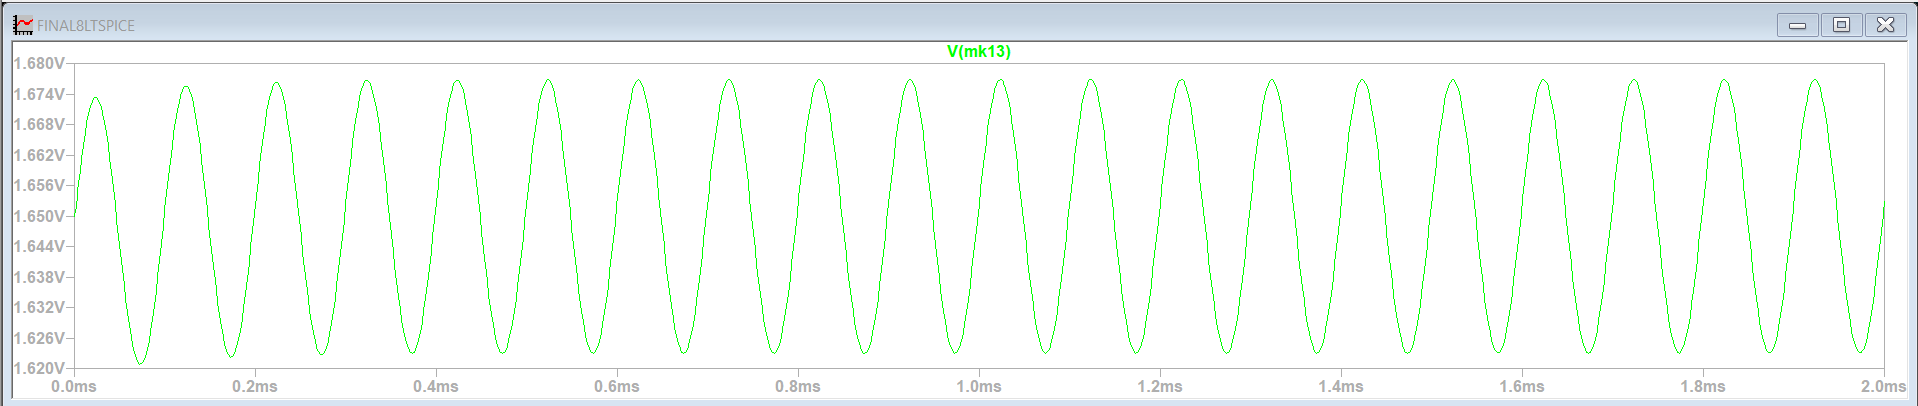
\includegraphics[width=1\linewidth]{imagess/voltage_700_70.png}
    \caption{Measured DUT voltage waveform.}
    \label{fig:eit_voltage}
\end{figure}

\begin{figure}[H]
    \centering
    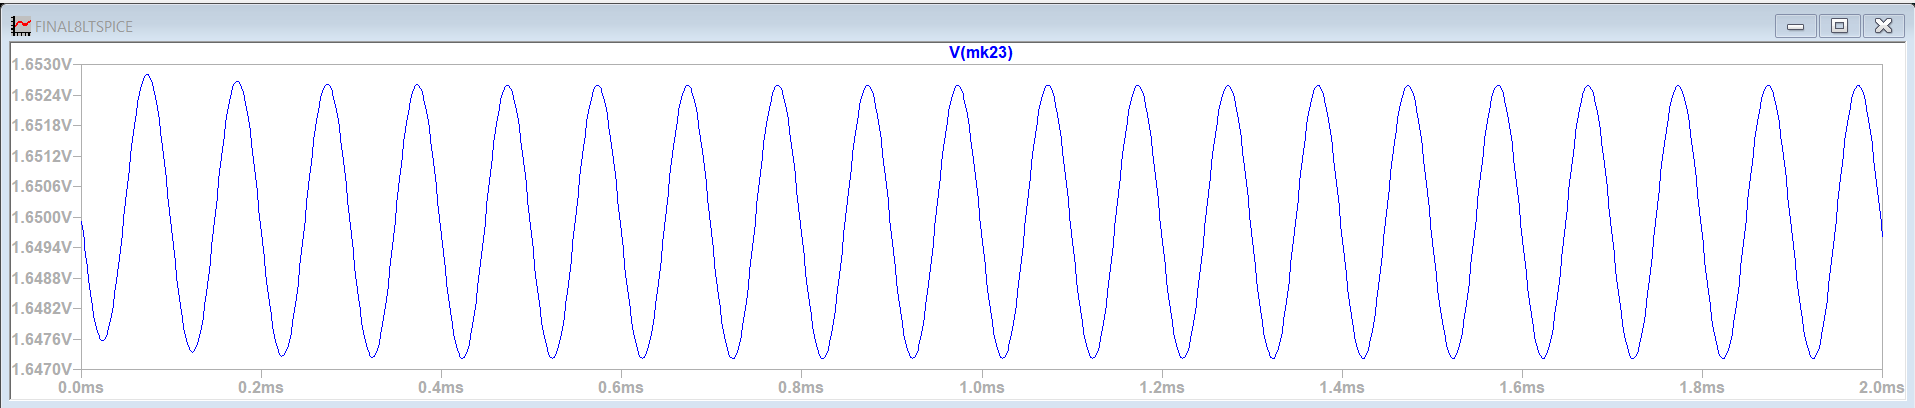
\includegraphics[width=1\linewidth]{imagess/current_700_70.png}
    \caption{Measured DUT current waveform obtained via shunt calculation.}
    \label{fig:eit_current}
\end{figure}
\subsubsection{Resistance calculation results}
The peak-to-peak current after shunt division is
\begin{equation}
I_\mathrm{pp} = \frac{V_\text{diff amplifier}}{R_\text{shunt}} = \frac{0.00539098~\mu\text{A}}{70~\Omega} \approx 77.014~\mu\text{A}.
\end{equation}
The peak-to-peak voltage measured across the DUT is
\[
V_\mathrm{pp} \approx 0.05351~\text{V}.
\]

\noindent Using the RMS relationship for a sinusoidal signal:
\[
V_\mathrm{rms} = \frac{V_\mathrm{pp}}{2\sqrt{2}}, \quad 
I_\mathrm{rms} = \frac{I_\mathrm{pp}}{2\sqrt{2}},
\]
the calculated resistance value confirms that the measurement chain correctly recovers the resistance value :
\begin{equation}
R_\text{calculated} = \frac{V_\mathrm{rms}}{I_\mathrm{rms}} 
= \frac{0.2680724 / (2\sqrt{2})}{382.905 \times 10^{-6} / (2\sqrt{2})} 
\approx 694.808~\Omega.
\end{equation}


The table bellow summarizes the time-domain validation results of the EIT acquisition system using single-frequency excitation. For each known resistor, the measured voltage and current were used to compute the effective resistance, The results show excellent agreement with the known resistance values, with minor deviations due to measurement precision and the finite resolution of the simulated acquisition circuit. For low-resistance loads, the measured current approaches the injected current limit, while for very high-resistance loads, the measured current is small, as expected. Overall, these results confirm that the simulation accurately reproduces the expected behavior of the resistive DUT, validating the correctness of the measurement chain.
\begin{table}[H]
\centering
\label{tab:single_freq_verification}
\begin{tabular}{|p{3cm}|p{3cm}|p{3cm}|p{3cm}|}
\hline
\textbf{Known resistance (\(\Omega\))} & \textbf{Measured Voltage (V)} & \textbf{Measured current (\(\mu\)A)} & \textbf{Calculated resistance (\(\Omega\))} \\ \hline
10  & 0.00433 & 431.7  & 10.029 \\ \hline
50  & 0.01692 & 341.0 & 49.619 \\ \hline
100  & 0.02686 & 270.0 & 99.481 \\ \hline
700  & 0.05351 & 77.014 & 694.808 \\ \hline
1000 & 0.05669 & 56.428 & 1004.643 \\ \hline
5000 & 0.06295 & 12.442 & 5059.475 \\ \hline
10000 & 0.06395 & 6.504 & 9832.410 \\ \hline
100000 & 0.06412 & 0.64657 & 99169.463 \\ \hline

\end{tabular}
\end{table}



\paragraph{(B) Frequency-domain Verification Using multi-frequency Excitation.}\\
The current injection was modeled using a behavioral current source configured to generate 
a multisine waveform composed of two frequency components. The injected current is given by  

\begin{equation}
I(t) = 100~\mu A \cdot \sin(2\pi \cdot 9765.625 \cdot t) 
     + 100~\mu A \cdot \sin(2\pi \cdot 49804.6875 \cdot t).
\end{equation}

This dual-tone excitation allows the system to be tested at two different frequency bands 
simultaneously, which is crucial for assessing multi-frequency EIT performance.
With multi-sine excitation, the complex impedance at each tone is estimated as
\begin{equation}
Z(f_k) \;=\; \frac{\mathcal{F}\{v(t)\}\big|_{f_k}}{\mathcal{F}\{i(t)\}\big|_{f_k}},
\quad
|Z(f_k)| = \frac{|V(f_k)|}{|I(f_k)|},\;
\angle Z(f_k) = \angle V(f_k) - \angle I(f_k),
\end{equation}
using the LTspice FFT on the voltage across and the current through the DUT. For a purely resistive load, \(|Z(f_k)| \approx R_\text{known}\) and \(\angle Z(f_k) \approx 0^\circ\) across tones (small deviations can occur from parasitics).\\
The time-domain waveforms for both the injected current and measured voltage are shown in the figures 3.15 and 3.16 . The multisine nature of the excitation is clearly visible in both signals, with the superposition of the two frequency components creating the characteristic beating pattern.
\begin{figure}[H]
    \centering
    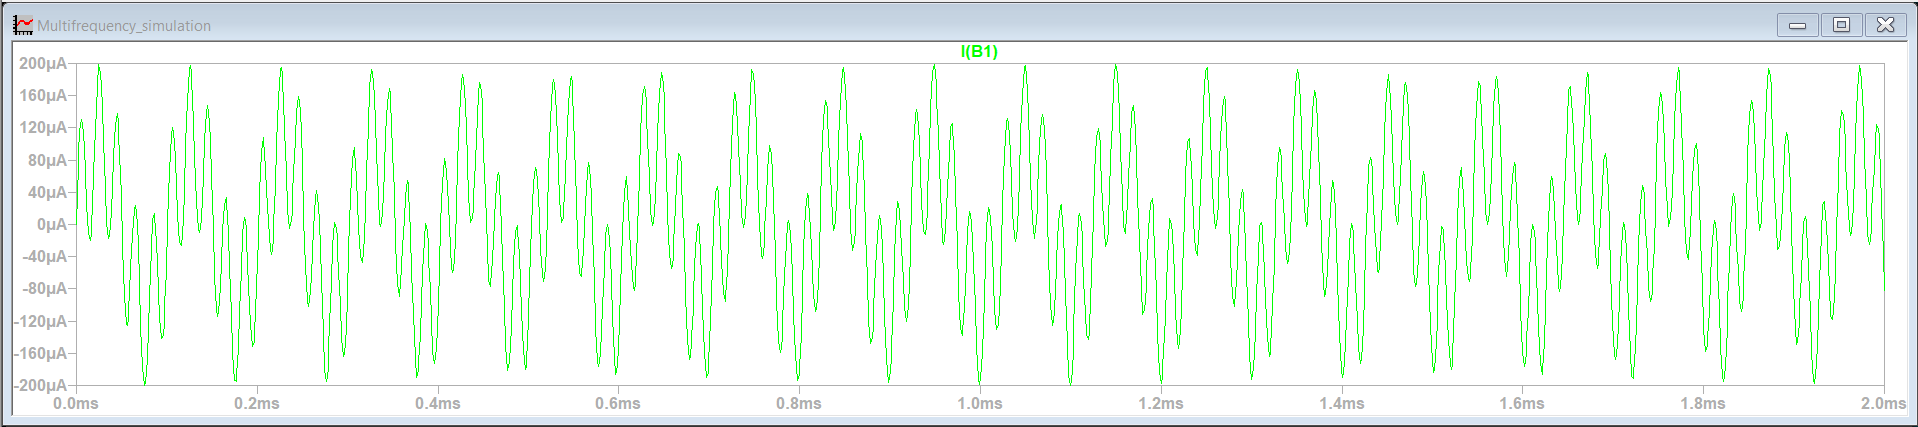
\includegraphics[width=1\textwidth]{imagess/injected_current_multifrequency.png}
    \caption{Injected current $I(t)$ .}
    \label{fig:current_time}
\end{figure}
\begin{figure}[H]
    \centering
    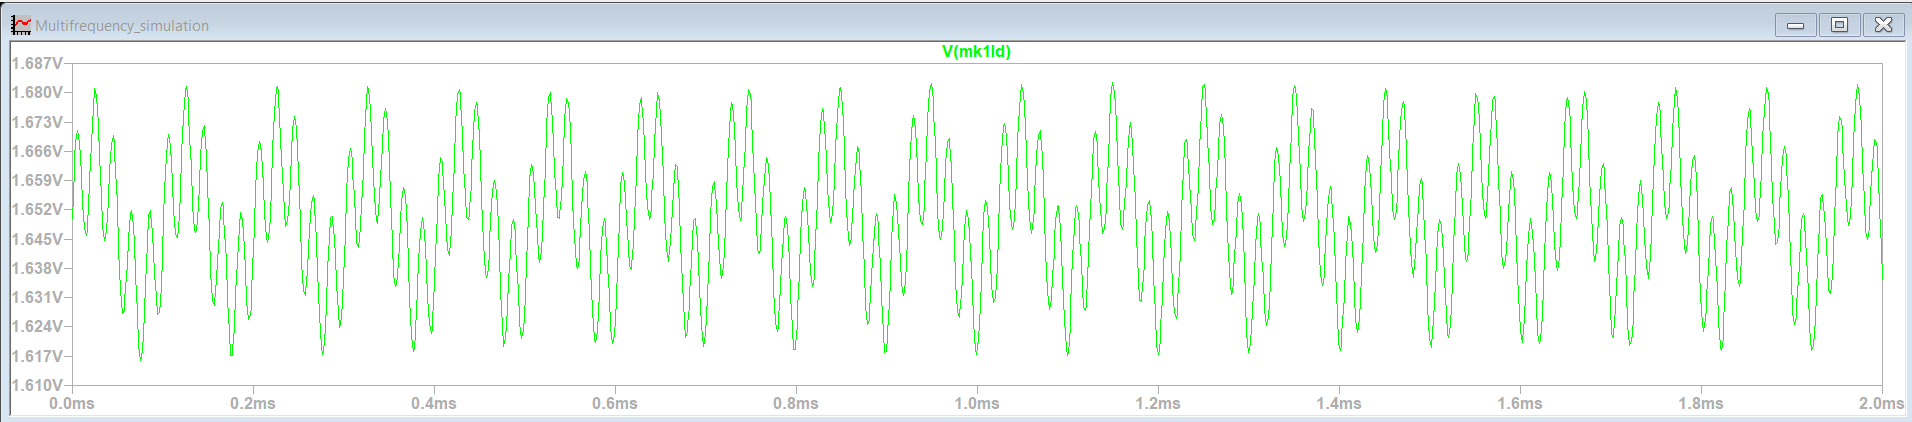
\includegraphics[width=1\textwidth]{imagess/voltage_multifrequency.png}
    \caption{Measured voltage $V(t)$.}
    \label{fig:voltage_time}
\end{figure}

The frequency-domain behavior of the simulated signals was analyzed using the Fast Fourier Transform (FFT). 
The spectra of the current and voltage waveforms exhibit distinct peaks at the two excitation frequencies, 
as shown in Figures~\ref{fig:fft_current} and~\ref{fig:fft_voltage}. 
The clean separation of frequency components confirms the effectiveness of the multisine excitation strategy 
for enabling simultaneous multi-frequency measurements.

\begin{figure}[H]
    \centering
    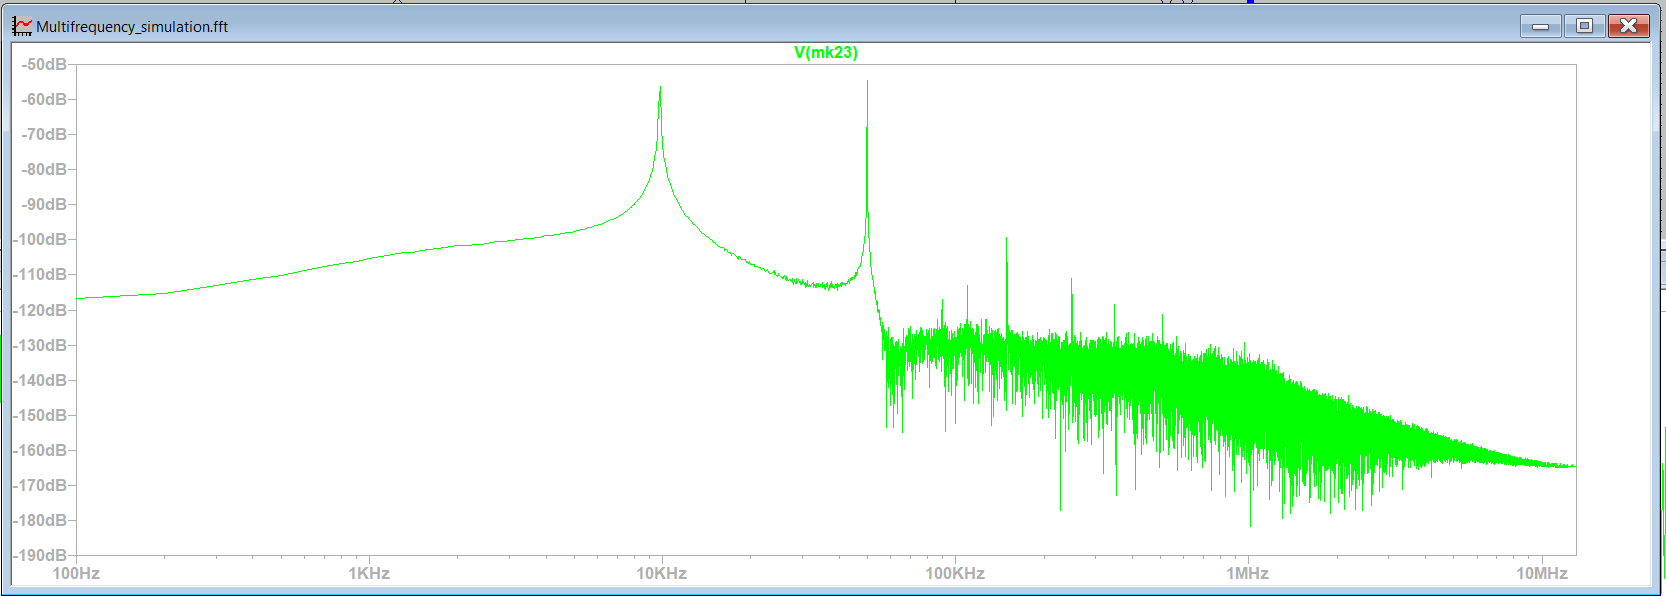
\includegraphics[width=0.9\textwidth]{imagess/FFT_ltspice_current.png}
    \caption{FFT spectrum of the simulated current signal.}
    \label{fig:fft_current}
\end{figure}

\begin{figure}[H]
    \centering
    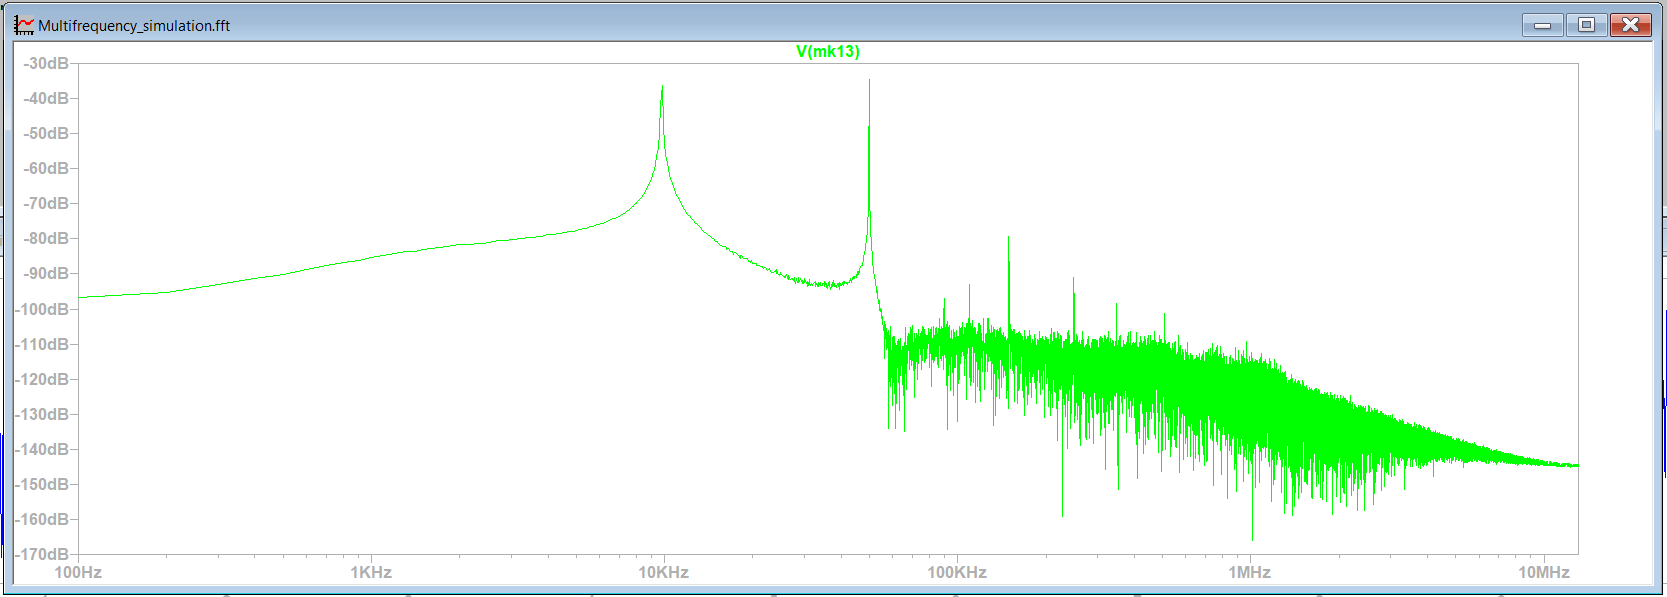
\includegraphics[width=0.9\textwidth]{imagess/FFt_ltspice_voltage.png}
    \caption{FFT spectrum of the simulated voltage signal.}
    \label{fig:fft_voltage}
\end{figure}


\subsubsection{Resistance calculation results}

To validate the impedance extraction methodology, a purely resistive reference load of 
$700~\Omega$ was implemented in LTspice. 
The current and voltage signals were processed via FFT, and the complex impedance was calculated. 
The resulting impedance values at the two excitation frequencies are summarized in Table~\ref{tab:impedance_results}.

\begin{table}[H]
    \centering
    \caption{Impedance extraction results from FFT analysis ($R_{\text{shunt}} = 70~\Omega$).}
    \label{tab:impedance_results}
    \begin{tabular}{|c|c|c|c|c|c|c|}
    \hline
    \textbf{Freq.} & \textbf{$|V(f)|$} & \textbf{$\angle V(f)$} & \textbf{$|I(f)|$} & \textbf{$\angle I(f)$} & \textbf{$|Z(f)|$} & \textbf{$\angle Z(f)$} \\
    \textbf{(kHz)} & \textbf{(mV)} & \textbf{(°)} & \textbf{($\mu$A)} & \textbf{(°)} & \textbf{($\Omega$)} & \textbf{(°)} \\
    \hline
    9.794  & 15.01 & -135.84 & 21.69 & 29.42 & 692.0 & -165.3 \\
    \hline
    49.802 & 18.14 & -92.00  & 24.51 & 81.19 & 740.1 & -173.2 \\
    \hline
    \end{tabular}
\end{table}

The extracted impedance magnitudes were $692.0~\Omega$ at 9.794~kHz and $740.1~\Omega$ at 49.802~kHz. 
These values are in close agreement with the theoretical $700~\Omega$ reference load, 
demonstrating the validity of the measurement chain. 
The small deviations in magnitude, together with the observed negative phase angles 
($-165.3^\circ$ and $-173.2^\circ$ instead of $0^\circ$), are attributed to numerical 
artifacts from the FFT process as well as parasitic elements inherent in the simulated setup.



The calculated values confirm that the expected $700~\Omega$ resistance is correctly 
recovered at both excitation frequencies. 
Importantly, since the two tones were applied simultaneously, this result validates not only the impedance 
extraction accuracy at individual frequencies but also the ability of the system to resolve 
multiple spectral components without crosstalk. 
This demonstrates that the FFT-based method can reliably extract impedance information in a 
simultaneous multi-frequency scenario, which is a key requirement for practical EIT systems. 
Consequently, this validation step establishes confidence in the measurement chain and provides 
a robust baseline before extending the approach to more complex DUTs and tissue-equivalent circuits.


\subsection{Circuit design}

After verifying the design through simulations, the circuit was implemented in EasyEDA to create an accurate schematic. The layout and connections were carefully checked to reduce unwanted parasitic effects that could affect high-frequency signal accuracy.

\begin{figure}[H]
    \centering
    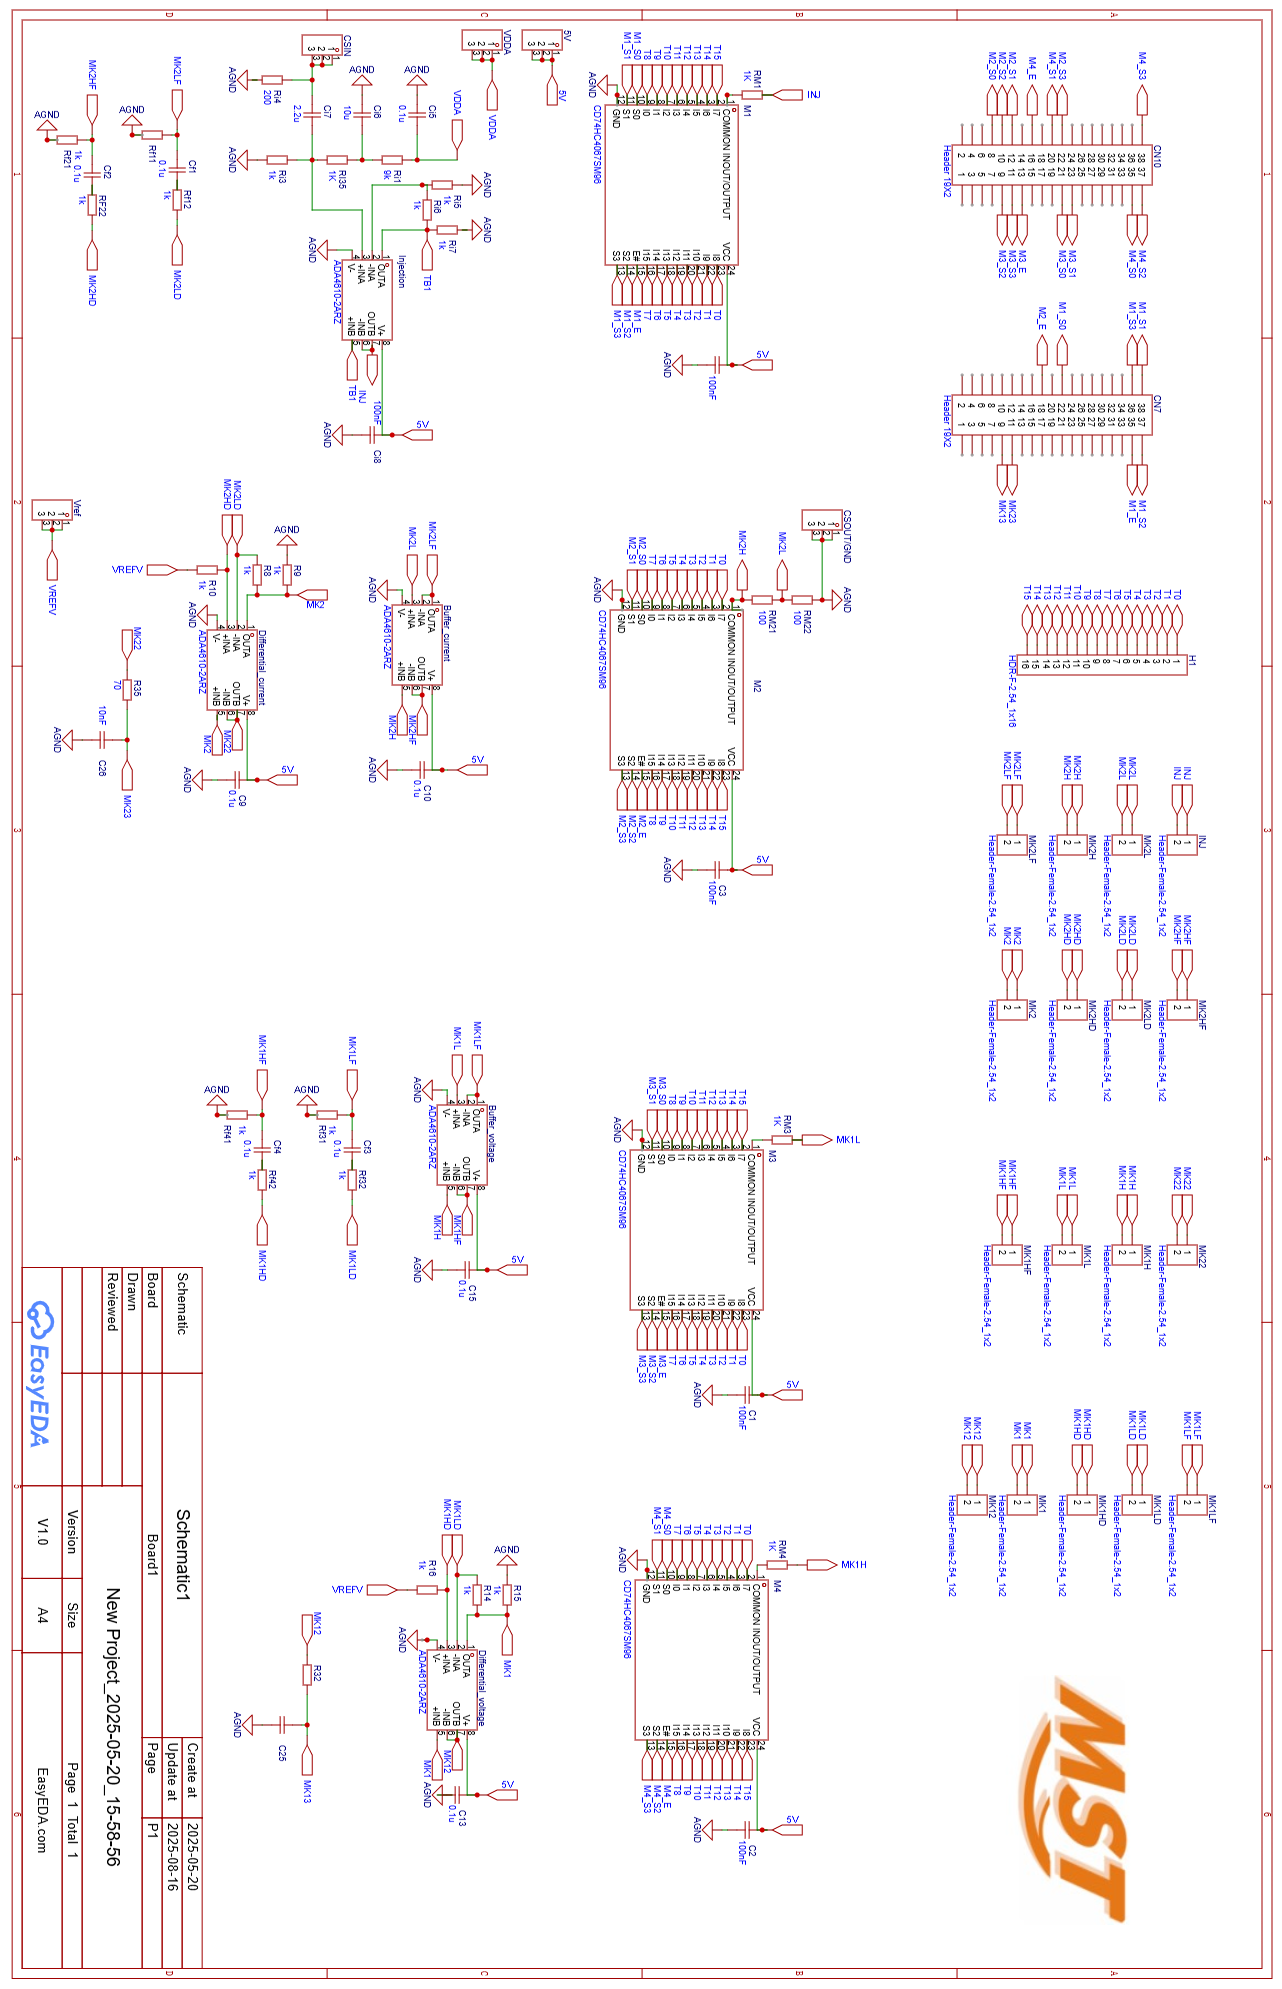
\includegraphics[width=0.8\textwidth]{imagess/SCH_Schematic1_1-P1_2025-08-16 (1).png}
    \caption{EasyEDA schematic of the EIT acquisition circuit.}
    \label{fig:easyeda_schematic}
\end{figure}

\subsection{PCB layout and routing}
  
The PCB layout was designed to minimize signal integrity, power supply stability, and noise, while not driving the overall size of the design up or making it unproducible. To achieve this, a two-layer PCB design was used, where one layer was completely utilized as a continuous ground plane and the second was utilized for the 5 V power plane and signal routing.

\begin{itemize}
    \item \textbf{Layer allocation:}  
    \begin{itemize}
        \item \textbf{Top layer:} Utilized solely as a continuous ground plane, providing a low-
impedance return path to every signal and suppression of electromagnetic inter-
ference (EMI). This also simplified grounding sensitive analog circuits and
shielding against switching noise.  
        \item \textbf{Bottom Layer:}Labeled as the 5 V distribution plane, it supported the main
supply rail with extra signal traces. The power was routed evenly around the
board, with high-current paths using wider traces.  
    \end{itemize}


    \item \textbf{Signal routing:}  
    Sensitive analog signals were routed with minimal trace length to
reduce susceptibility to pickup by noise. Traces were taken wherever possible directly
over the solid ground plane for controlled impedance and reduced loop areas.
High-frequency excitation signals were careful routed to avoid crosstalk, and digital lines
were not routed parallel to each other.

    \item \textbf{Power integrity and decoupling:}  
    Power Integrity and Decoupling: Since the 5 V supply was delivered by the bottom plane, local decoupling capacitors were placed near each component (e.g.,
the microcontroller, op-amps, and voltage regulator) in stabilizing the voltage at the current point of load and in removing transient oscillations. Bulk capacitors were distributed across near the power input connector to ensure stable operation under sustained dynamic load conditions.  

    \item \textbf{Grounding strategy:}  
    A complete dedicated ground plane layer was used to provide short and direct path for all components to reference potential and keep ground noise to a minimum. This reduced ground loops and optimized overall signal quality. 

    \item \textbf{Design rule checks (DRC):}  
    Layout was verified to meet the PCB manufacturer's trace width, clearance, via size, and annular ring requirements, ensuring fabrication-free trouble.
    \item \textbf{Tool and Visualization:}  
  Tool and Visualization: The PCB was designed and verified using EasyEDA, providing both electric rule checking and advanced visualization capabilities. \\

\end{itemize}
Figure~\ref{fig:pcb_all} presents the complete design of the PCB in EasyEDA, including both the top and bottom layer routings as well as the corresponding 3D views.
\begin{figure}[H]
    \centering
    % (a) Top layer PCB
    \begin{subfigure}[b]{0.45\textwidth}
        \centering
        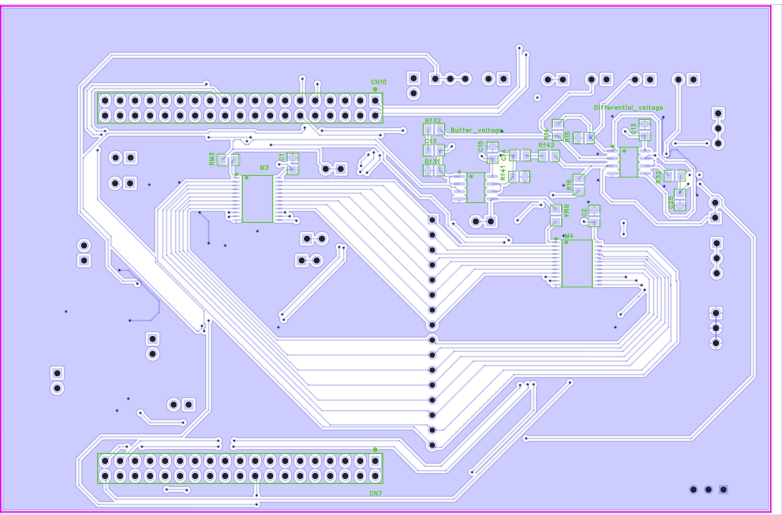
\includegraphics[width=\textwidth]{imagess/top_layer.jpg}
        \caption{PCB layout and routing (top layer view).}
        \label{fig:pcb_layout3}
    \end{subfigure}
    \hfill
    % (b) Bottom layer PCB
    \begin{subfigure}[b]{0.45\textwidth}
        \centering
        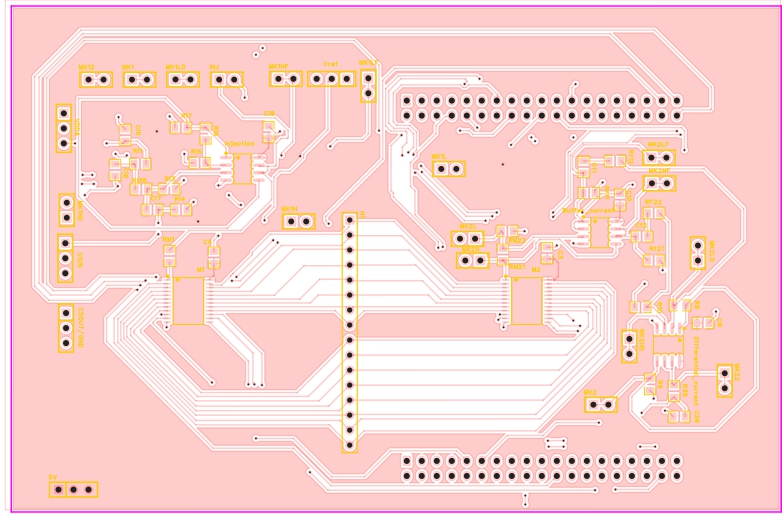
\includegraphics[width=\textwidth]{imagess/PCB_PCB1_2025-08-17 (1)_page-0001.jpg}
        \caption{PCB layout and routing (bottom layer view).}
        \label{fig:pcb_layout4}
    \end{subfigure}
    
    \vspace{0.5cm} % spacing between rows
    
    % (c) 3D Top view
    \begin{subfigure}[b]{0.45\textwidth}
        \centering
        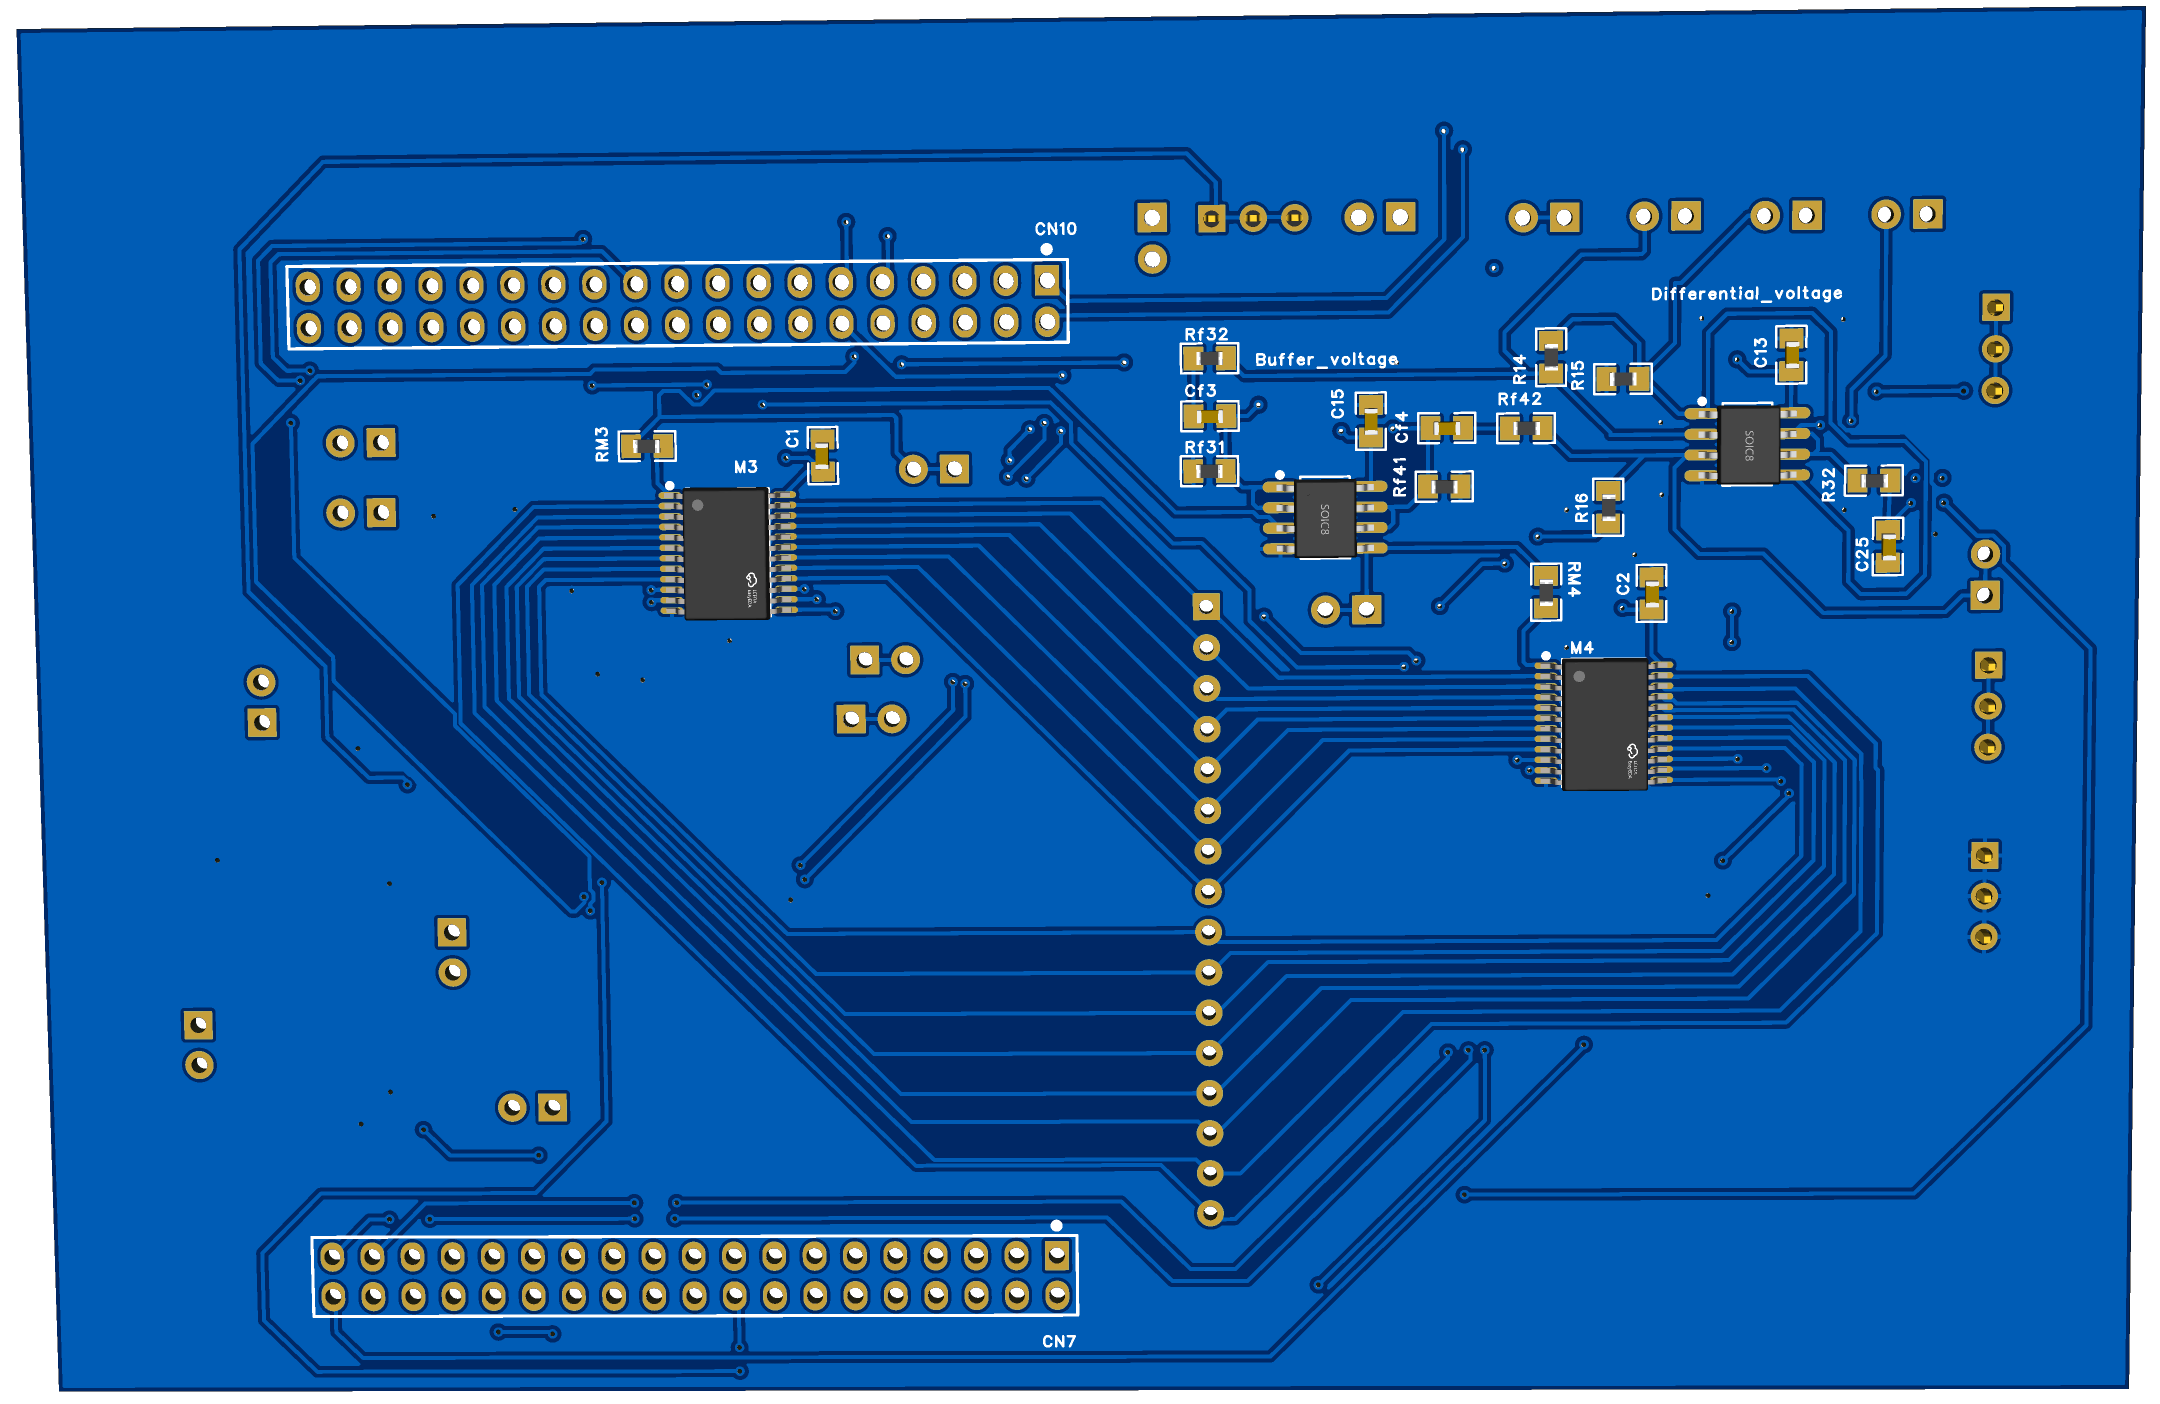
\includegraphics[width=\textwidth]{imagess/3D_PCB1_2025-07-16 (1).png}
        \caption{3D layout (top view).}
        \label{fig:pcb_layout}
    \end{subfigure}
    \hfill
    % (d) 3D Bottom view
    \begin{subfigure}[b]{0.45\textwidth}
        \centering
        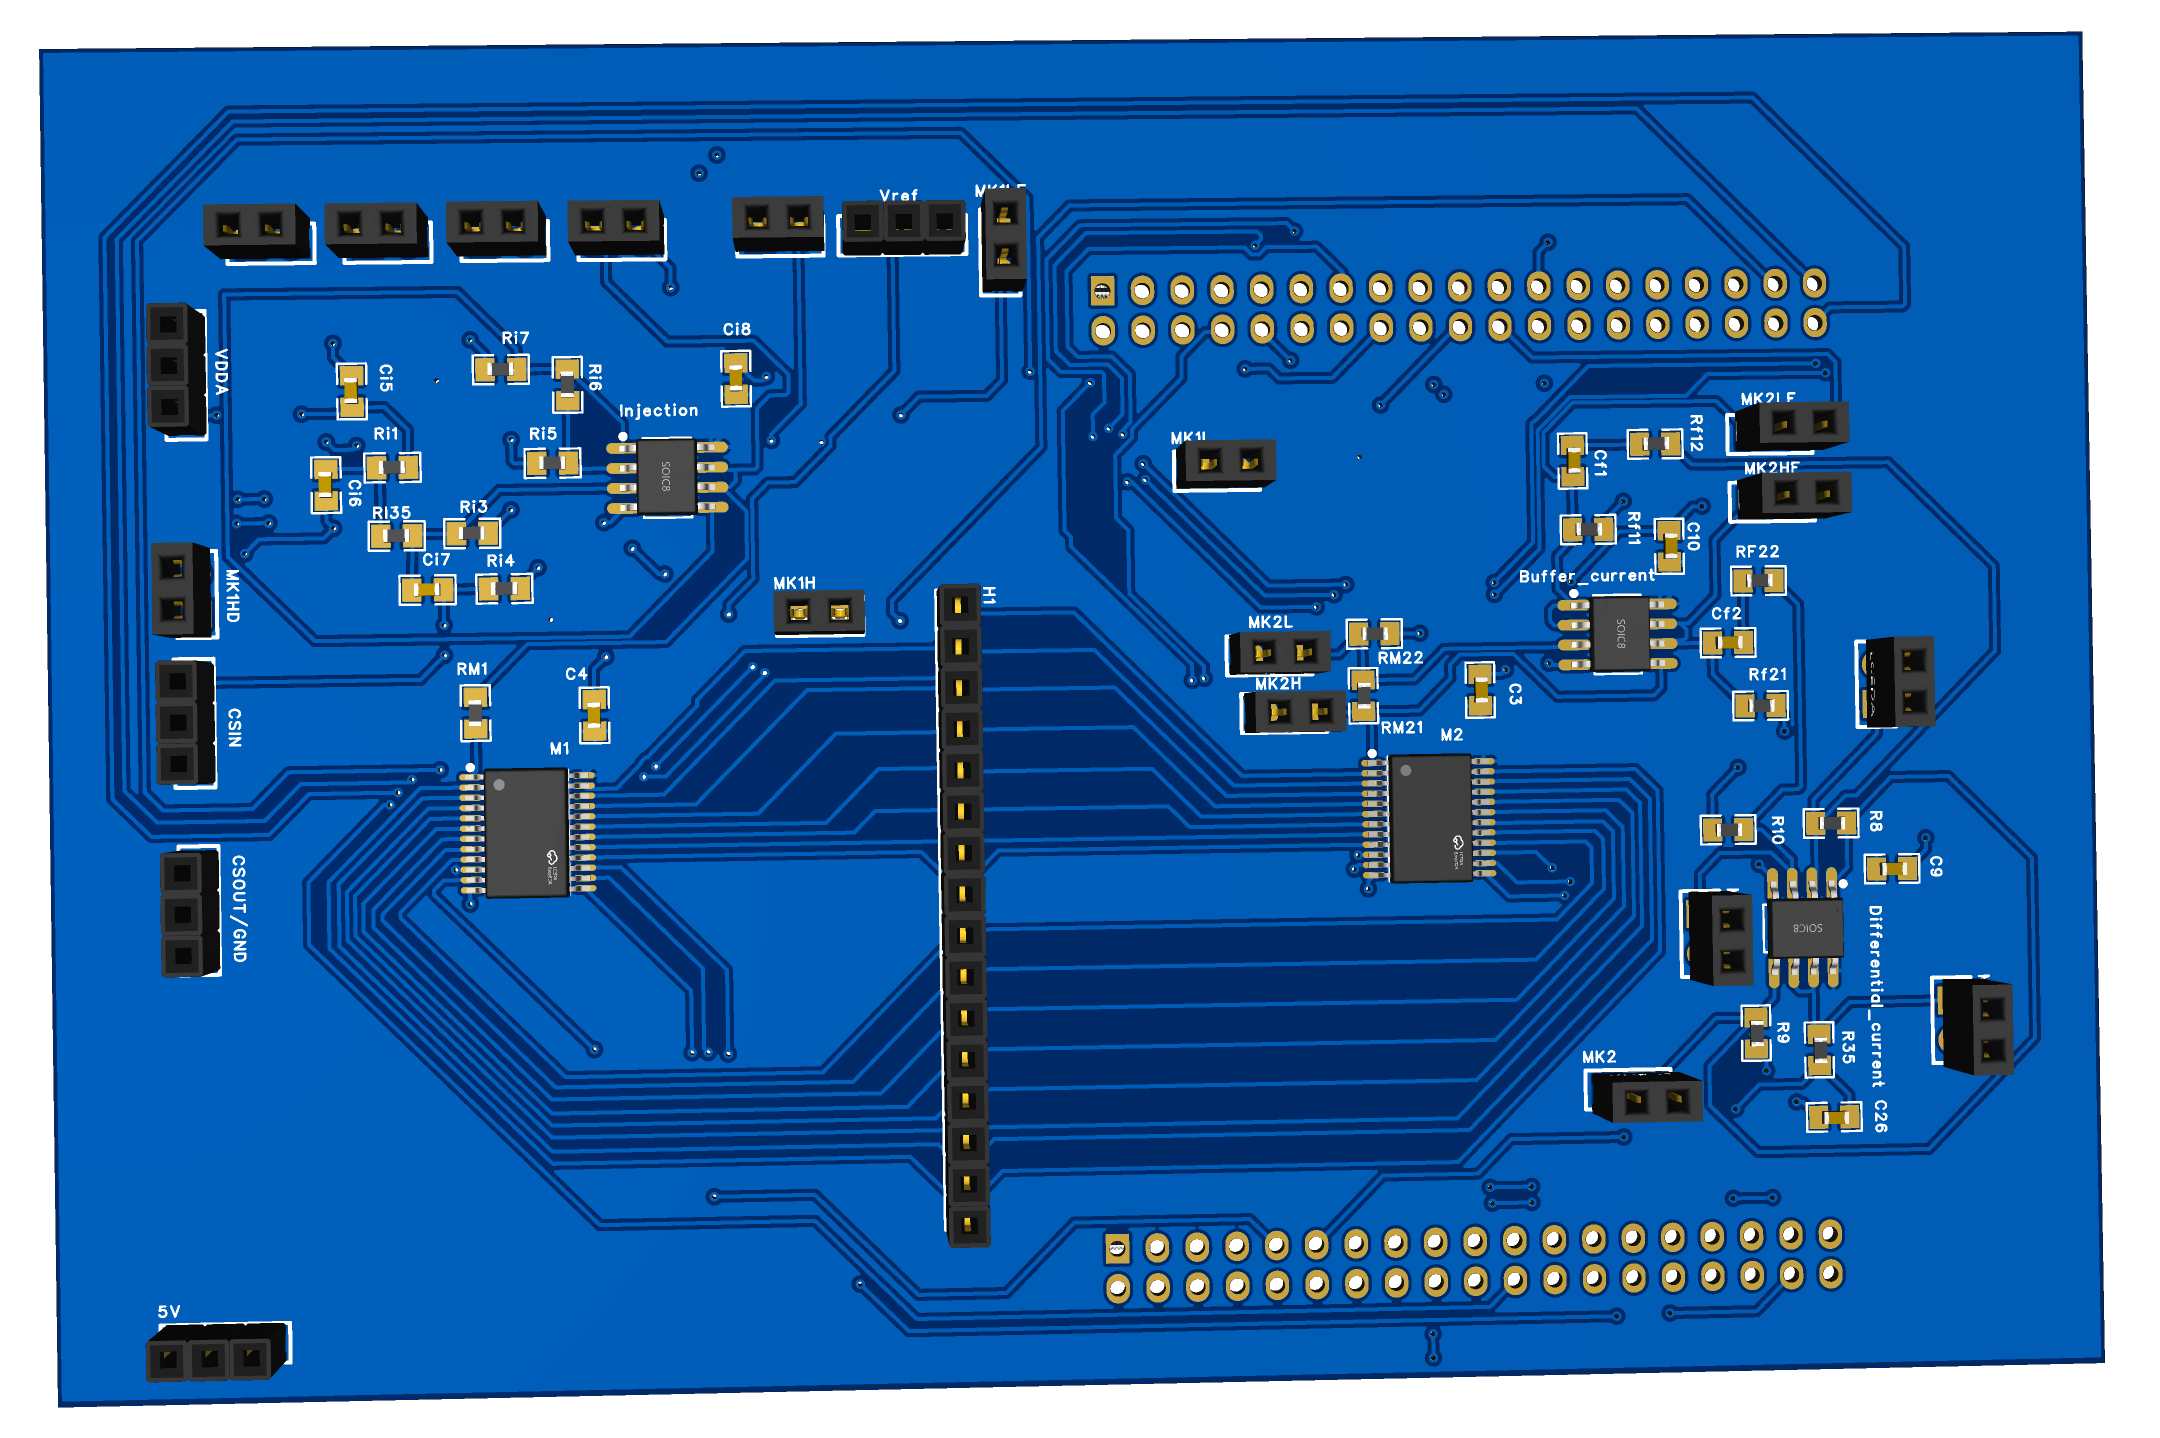
\includegraphics[width=\textwidth]{imagess/3D_PCB1_2025-08-16 (2).png}
        \caption{3D layout (bottom view).}
        \label{fig:pcb_layout2}
    \end{subfigure}
    
    \caption{PCB layouts and 3D views in EasyEDA: (a) top layer routing, (b) bottom layer routing, (c) 3D top view, (d) 3D bottom view.}
    \label{fig:pcb_all}
\end{figure}
\subsection{Generation of manufacturing documentation } 
  Figure~\ref{fig:drc} shows the rule configuration inside EasyEDA.

\begin{figure}[H]
\centering
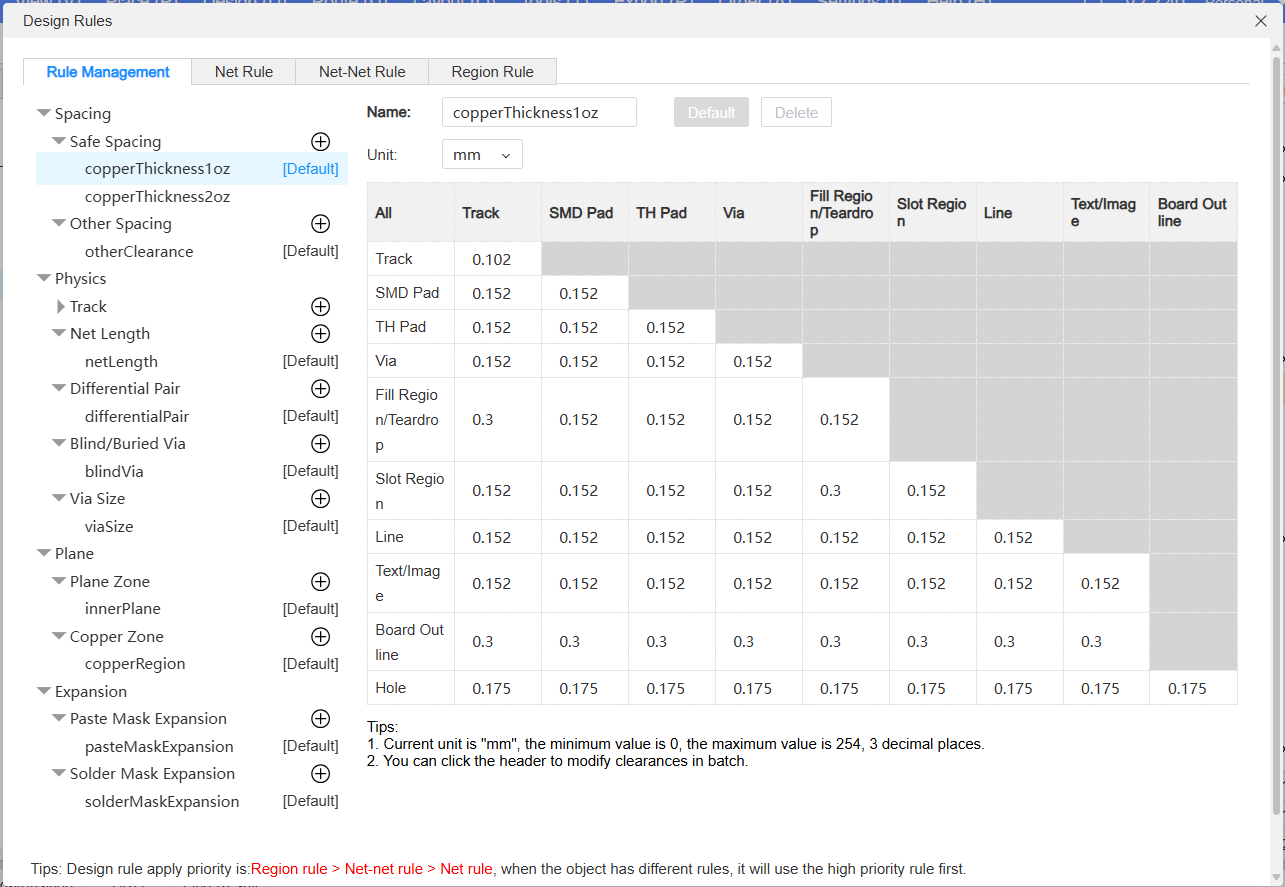
\includegraphics[width=0.6\textwidth]{imagess/Screenshot 2025-08-17 104409.png}
\caption{Design rule settings in EasyEDA aligned with Fischer’s manufacturing constraints.}
\label{fig:drc}
\end{figure}

After validating the design with the DRC tool, the Gerber and BOM files were generated and subsequently uploaded to Fischer’s online platform. This ensured that the board specifications sizes were fully compatible with the manufacturer’s production capabilities, guaranteeing reliable and reproducible fabrication.

\begin{table}[H]
\centering
\caption{Fischer PCB Manufacturing Rules for 2-Layer Boards\cite{FischerPCB}}
\begin{tabular}{|c|c|c|}
\hline
\textbf{Copper Thickness} & \textbf{Min. Trace Width} & \textbf{Min. Spacing} \\
\hline
35\,µm (1 oz)  & 150\,µm (6 mil)  & 150\,µm (6 mil) \\
\hline
70\,µm (2 oz)  & 200\,µm (8 mil)  & 200\,µm (8 mil) \\
\hline
105\,µm (3 oz) & 300\,µm (12 mil) & 350\,µm (14 mil) \\
\hline
\multicolumn{3}{|c|}{\textbf{Minimum finished drill diameter: 0.3\,mm}} \\
\hline
\end{tabular}
\end{table}
\section{STM32-based excitation and acquisition}

This section presents the embedded system implementation on the STM32 microcontroller, 
covering the generation of excitation signals, multiplexer control, and synchronized 
data acquisition. Screenshots from STM32CubeMX, oscilloscope captures, and configuration 
parameters are provided to illustrate the design.  

\subsection{Excitation signal generation}

The excitation signal was generated using the \textbf{DAC peripheral}, driven by a timer 
(\texttt{TIMx}) to ensure deterministic sampling. The DAC waveform was based on a 
precomputed sine lookup table stored in memory.  

To satisfy the Nyquist criterion and ensure accurate waveform synthesis, the sampling 
frequency was chosen to be at least 2 times higher than the maximum excitation frequency 
of 500~kHz, resulting in a DAC sampling rate of $\geq 1$~MHz.  

The timer frequency was computed as\cite {ST_RM0090}:  

\begin{equation}
f_{\text{timer}} = \frac{f_{\text{clk}}}{(PSC+1)(ARR+1)}
\end{equation}


where $f_{\text{clk}}$ is the system clock frequency, $PSC$ is the prescaler value, and $ARR$ 
is the auto-reload register value.  

\subsubsection*{Parameters}
\begin{itemize}
    \item Prescaler (PSC): \texttt{1}
    \item Auto-reload register (ARR): \texttt{39}
    \item Resulting timer frequency: \texttt{1M} Hz
    \item DAC resolution: 12-bit
\end{itemize}

\end{figure}
To acquire both the voltage and current signals simultaneously, two ADC channels were configured: \texttt{ADC1} for voltage measurement and \texttt{ADC2} for current measurement. In order to guarantee synchronization between the two channels, both were triggered by the same timer (\texttt{Timer~2}). This ensures that the sampling of voltage and current occurs at exactly the same instants, which is crucial for accurate impedance reconstruction.

To further optimize the acquisition process, Direct Memory Access (DMA) was enabled. The use of DMA allows the sampled data from both ADCs to be transferred directly into memory without CPU intervention, thereby improving system efficiency and reducing latency.





The ADC channels were sampled using the STM32 HAL library. To start the acquisition, the ADCs were first calibrated, then started in DMA mode, and finally triggered by Timer~2. This process was implemented through the following functions:


\begin{itemize}
    \item \texttt{HAL\_ADCEx\_Calibration\_Start} performs a single-ended calibration of ADC1.
    \item \texttt{HAL\_ADC\_Start\_DMA} starts the ADC in DMA mode, storing 1024 samples into \\\texttt{adcValueArray}.
    \item \texttt{HAL\_TIM\_Base\_Start} starts Timer~2, which triggers the ADC at the configured sampling frequency of 5~MHz.
\end{itemize}

\subsection{Injection control}
The electrode switching module is a crucial part of the EIT system. The number of electrodes directly impacts several key aspects of the EIT system, such as measurement speed, computational load for image reconstruction, and image resolution. Commonly used configurations in EIT systems include 8, 16, 32, or 64 electrodes. Systems with fewer electrodes offer simpler and more reliable hardware designs but result in lower imaging resolution and reduced detail in reconstructed images. Conversely, systems with a larger number of electrodes, such as 64, can acquire more measurement data, improving imaging quality. However, this also leads to longer acquisition times, which may restrict the system’s practical applications.

Considering these trade-offs, a 16-electrode configuration was selected for this work. This choice provides a balanced compromise between hardware complexity, system reliability, and imaging performance.

In any EIT system, both the current injection electrodes and the voltage measurement electrodes need to be switched rapidly and accurately. Multiplexers are used to perform this switching. 

Each multiplexer has five control inputs: the enable pin (\texttt{E}) and four selection bits (\texttt{S0-S3}), which allow access to all 16 channels. For this design, four multiplexers are used in total: two for the current injection electrodes and two for the voltage measurement electrodes. Controlling these four multiplexers requires 20 GPIO pins. The STM32G4 microcontroller used in this project has 144 available pins, allowing sufficient resources to manage all multiplexers along with other required functions.
Four analog multiplexers were programmed through GPIO pins. A control algorithm cycles 
through electrode pairs in an adjacent injection pattern. 


The logic is implemented using nested loops, as illustrated in Figure~\ref{fig:adjacent_injection}.
\begin{figure}[H]
    \centering
    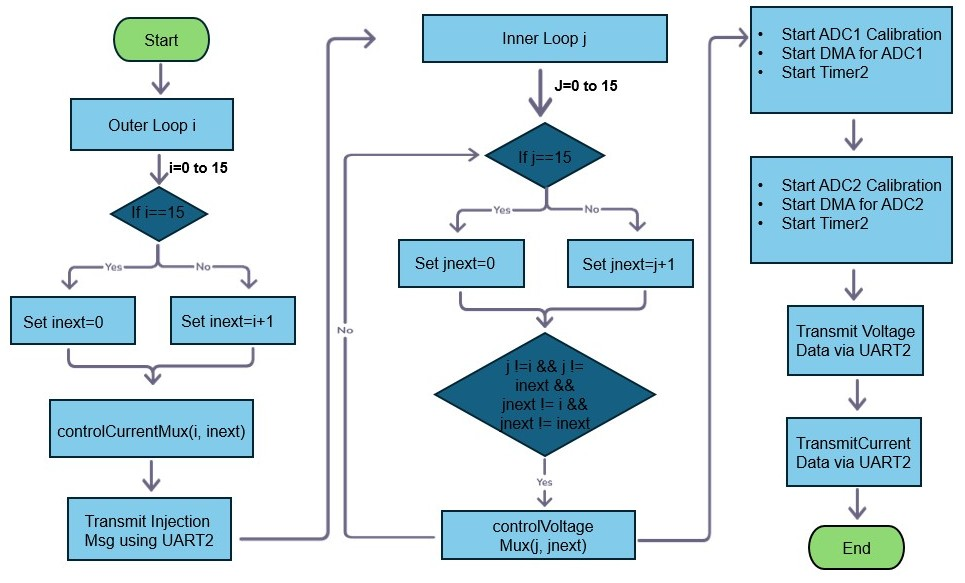
\includegraphics[width=1\textwidth]{imagess/injection_diagram.jpg}
    \caption{Diagram of adjacent electrode injection scheme using 4 multiplexers.}
    \label{fig:adjacent_injection}
\end{figure}

\begin{itemize}
    \item \textbf{Outer loop (\texttt{i})}: selects the current injection pair.
    \item \textbf{Inner loop (\texttt{j})}: controls the voltage measurement channels.
    \item The \texttt{inext} index ensures adjacent injection, wrapping around the electrodes:
    \[
    \texttt{inext} = 
    \begin{cases}
    0 & \text{if } i = 15 \\
    i+1 & \text{otherwise}
    \end{cases}
    \]
\end{itemize}

Two control functions were implemented in the firmware to manage this switching:

\begin{itemize}
    \item \texttt{controlCurrentMux(int channelIn, int channelOut)}  
    This function configures the multiplexers that connect the current source to the selected electrode pair. The parameters \texttt{channelIn} and \texttt{channelOut} correspond to the indices of the input and output electrodes, respectively. Each multiplexer address line (S0--S3) is driven by the STM32 GPIO pins using the \texttt{HAL\_GPIO\_WritePin()} function, which sets the binary control word according to the desired channel index:
    \[
    \text{MUX Address} = \bigl[b_3\; b_2\; b_1\; b_0 \bigr] \quad \Rightarrow \quad \text{Selected Electrode Channel}.
    \]

    \item \texttt{controlVoltageMux(int channelIn, int channelOut)}  
    This function operates in the same way, but for the voltage measurement electrodes. The input electrode (\texttt{channelIn}) and output electrode (\texttt{channelOut}) are selected through two multiplexers, with their address bits written via the microcontroller GPIO pins. This allows the system to measure the differential boundary voltage across the chosen electrode pair.
\end{itemize}

By abstracting the multiplexer control into these two functions, the electrode selection process becomes modular and easily programmable. During a full EIT measurement cycle, the firmware iterates through predefined electrode configurations, sequentially activating the appropriate pairs for current injection and voltage measurement. This automated switching is essential for reconstructing tomographic images, as it enables systematic data collection across all electrode combinations without manual reconfiguration.





\section{ Conclusion}
In this chapter, the process of designing the PCB was described in detail from layout, routing, design rule check, generation of Gerber and BOM files for safe man-
ufacturing. The STM32-based excitation and acquisition unit was installed,
encompassing DAC signal generation, multiplexer-driven electrode switching, and
synchronized ADC data acquisition. The 16-electrode configuration adopted
strikes a hardware complexity and imaging performance compromise, allowing for
systematic and automated data collection for EIT measurements.
